\section[Datenblatt Signalgenerator]{Datenblatt des DDS-Signalgenerators}



\begin{minipage}{0.4\textwidth}
\begin{flushleft}
\subsection{Features}
Der Signalgenerator basiert auf dem Prinzip der Direkten Digitalen Synthese (DDS) und ist in der Lage, Ausgangs ein breites Spektrum an Frequenzen, Signalformen und Ausgangsspannungen zu erzeugen. Die Steuerung des Gerätes erfolgt ausschließlich über den Computer, ein autarker Betrieb ist möglich. Im Gerät können hardwarespezifische Kalibrierungswerte gespeichert werden.
\end{flushleft}
\end{minipage}
\hfill
\begin{minipage}{0.58\textwidth}
\begin{flushright}
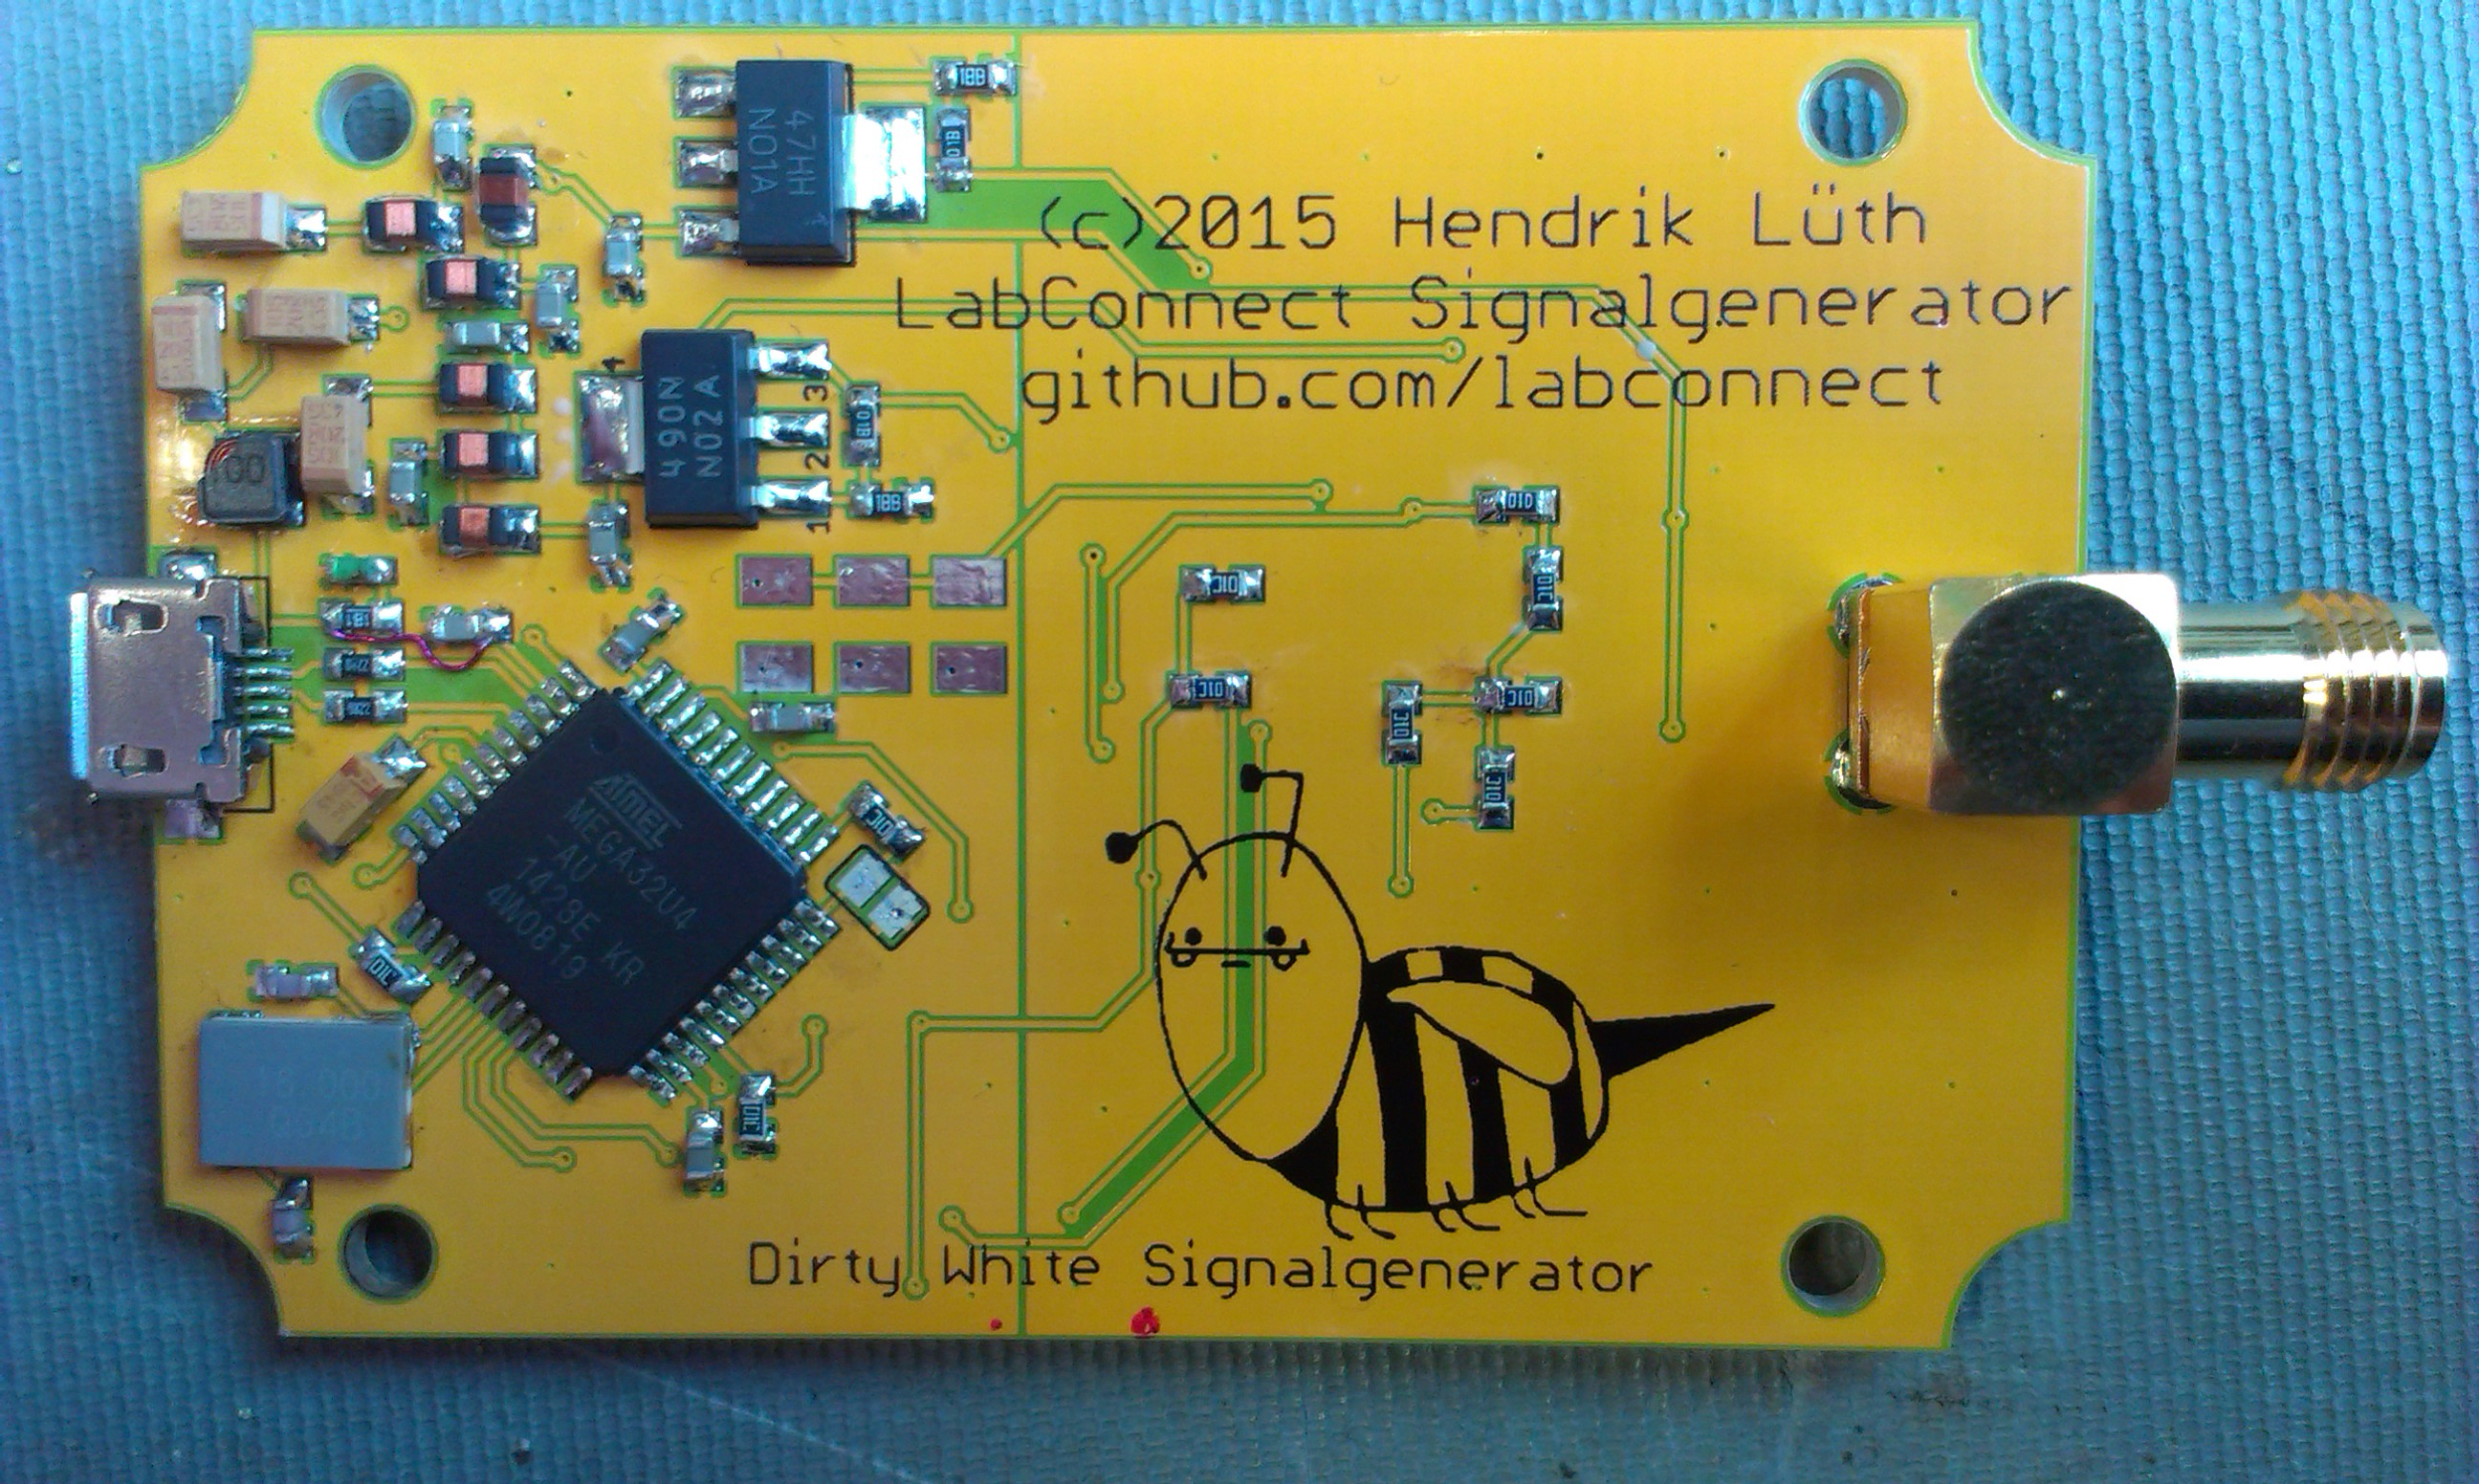
\includegraphics[width=\textwidth]{./img/FotoSgen.jpg}
\end{flushright}
\end{minipage}
\subsection{Eigenschaften}
\begin{center}
\begin{tabular}{l|ccc|c|l}
\hline
\textbf{Parameter} & \textbf{~~Min~~} & \textbf{~~Typ~~} & \textbf{~~Max~~} & \textbf{Einheit} & \textbf{Testbedingungen} \\
\hline
Betriebsspannung $U_{B}$ & 4,7 & 5 & 5,5 & Volt & \\
Stromaufnahme $I_{ges.}$ & 30 & 50 & 100 & mA & $U_{B}$=5V \\
Leistungsaufnahme P & 0,14 & 0,25 & 0,55 & W & \\
\hline
\end{tabular}
\end{center}

\subsection{Absolute Maximum Ratings}
\begin{center}
\begin{tabular}{l|c|c}
\hline
\textbf{Parameter} & \textbf{~~Max~~} & \textbf{Einheit} \\
\hline
Betriebsspannung $U_{B}$ & 6 & Volt \\
Spannung an D+ $U_{D+}$ & 3,6 & Volt \\
Spannung an D- $U_{D-}$ & 3,6 & Volt \\
\hline
Ausgangsstrom $I_{a}$ & 95 & mA \\
\end{tabular}
\end{center}
